\chapter{Visão Geral}

Para embasar e planejar o projeto a ser desenvolvido, uma proposta de
arquitetura precisa ser feito. Neste capítulo será apresentado a proposta do projeto UMISS,
sendo explanado as arquiteturas de cada subsistema.

\section{Subsistema - Processamento de Sinais e Monitoramento}

O subsistema de controle e monitoramento terá como grande objetivo a aquisição
dos sinais do paciente, a disponibilização desses recursos para os
interessados, e a notificação dos responsáveis em casos de eventos críticos.
Sua arquitetura pode ser dividido em três grandes
módulos: o módulo que chamaremos \textbf{módulo eletrônico}, que conterá
grande parte dos componentes eletrônicos do projeto,
o \textbf{módulo servidor remoto}, que será um servidor remoto disponível
para ser consumido por outros serviços, e o \textbf{módulo aplicativo},
que será uma solução em aplicativo para ser utilizado pelos interessados.

\subsection{Módulo Eletrônico}
O módulo eletrônico será composto principalmente por sensores, amplificadores,
filtros, conversores, e um sistema embarcado.

Os sensores terão como principal papel a extração dos sinais vitais do
paciente, e serão acoplados a estrutura da cadeira, de forma que algum
membro do paciente fique em contato com o sensor, permitindo assim a
aquisição do sinal.

Os amplificadores e filtros serão responsáveis pelo tratamento do sinal;
amplificadores tendo o papel de aumentar o ganho extraído pelo sinal,
e os filtros tendo o papel de atenuar ruídos capturados.

Os conversores terão como papel a conversão dos sinais tratados para um formato
que o sistema embarcado possa entender; no caso do projeto UMISS, a conversão
a ser feita será de analógica para digital.

Um sistema embarcado será responsável por receber os sinais do paciente,
processá-los e utilizá-los em tarefas específicas, e, por fim, despachar os
dados para o módulo servidor remoto.

\subsection{Módulo Servidor Remoto}
O módulo servidor remoto é dividido nos seguintes componentes: um servidor remoto
e gerência de configuração do servidor.

O servidor remoto será um servidor hospedado fora da rede-interna da parte
eletrônica, e poderá ser acessado via \textit{internet}. Se comunicará com
o sistema embarcado da parte eletrônica utilizando comunicação
\textit{via socket}\footnote{\url{https://docs.oracle.com/javase/tutorial/networking/sockets/definition.html}},
apresentará dados para o aplicativo, e o notificará da ocorrência de eventos
críticos.

A gerência de configuração do servidor será composta principalmente de
configurações e \textit{scripts} que vão permitir a manutenção e
interoperabilidade entre o servidor e outros recursos.

\subsection{Módulo aplicativo}

O aplicativo só tem si próprio como componente, e será utilizado regularmente
pelos responsáveis do paciente; estará preparado para receber as notificações
do servidor e para mostrar os dados em tempo real.

\subsection{Integração entre os módulos}

\begin{figure}[H]
  \centering
    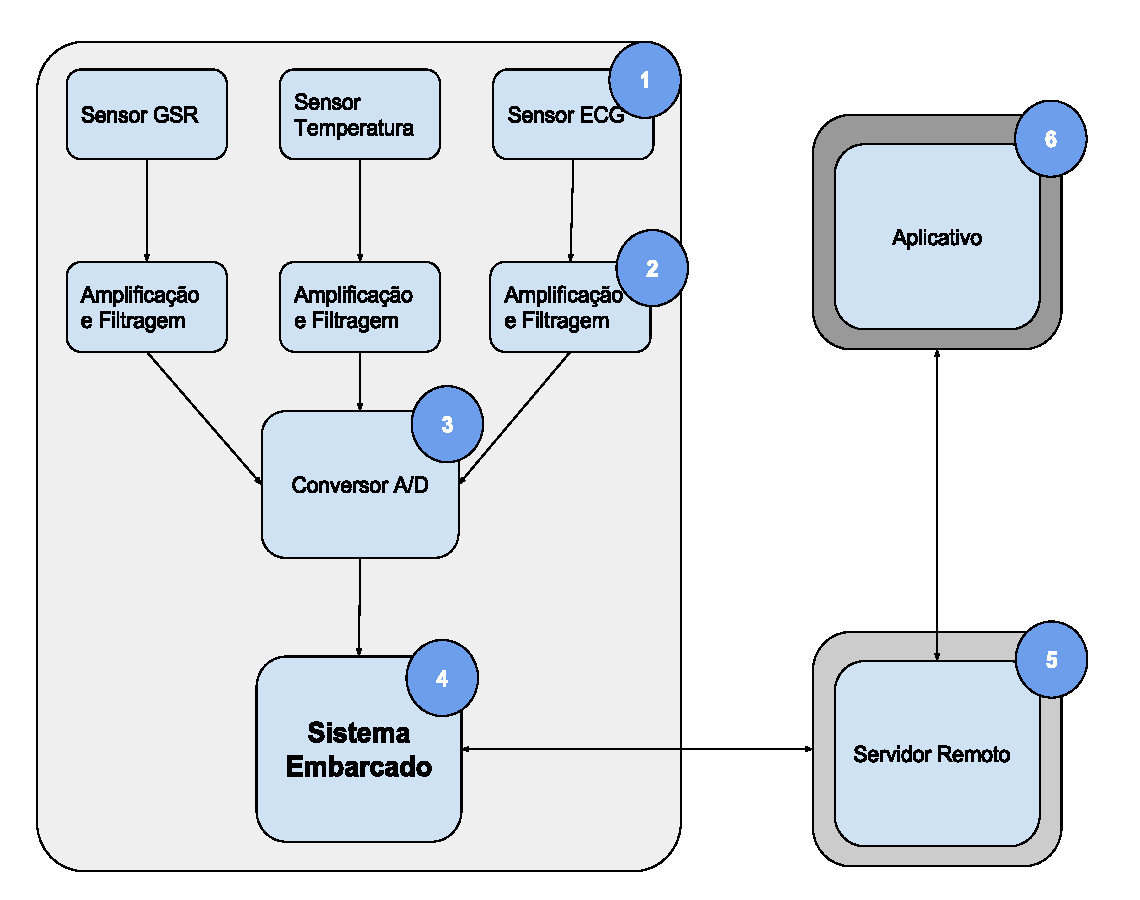
\includegraphics[width=\textwidth]{figuras/arquitetura-monitoramentoecontrole.eps}
  \caption{Fluxo típico do subsistema de Monitoramento e Controle}
  \label{fig:arquitetura-monitoramento-e-controle}
\end{figure}

O passo (1) do subsistema é atuado pelos sensores, que extraírão sinais do paciente;
o passo (2) será atuado pelos amplificadores e filtros, e tratarão o sinal
extraído pelos sensores no passo anterior; no passo (3) os sinais tratados
são convertidos para formato digital, para que possam ser lidos pelo sistema
embarcado; no passo (4) o sistema embarcado recebe as informações do conversor
e abre conexão com o servidor remoto - após, envia as informações recebidas,
quando necessário; no passo (5) o servidor remoto recebe dados do sistema
embarcado e passa informações importantes para o aplicativo, e, por fim,
no passo (6), o aplicativo recebe as informações.

\subsection{Tecnologias Utilizadas}

\subsubsection{Servidor Django}
\label{sub:servidor_django}
O passo (5), retratado na Figura \ref{fig:arquitetura-monitoramento-e-controle},
representa o servidor remoto, que irá receber as informações de todas as
estações embarcadas do sistema. Este será responsável por receber, processar
e se comunicar com os dispositivos móveis cadastrados no sistema. Para tal,
será utilizado uma linguagem de programação compatível com a que será utilizada
no software embarcado, que será escrito em python. Desta maneira, todo
o servidor proverá serviços utilizando python.

Um Framework robusto e já bastante consolidado na comunidade python é o Django.
Este é bem completo e possui várias ferramentas que auxiliam no desenvolvimento.
O django possui um framework para API's Rest, que será o padrão utilizado pelos
clientes para se comunicarem, chamado de DjangoRestFramework. Este é muito poderoso
e de alta produtividade.

Estas três ferramentas irão compor juntas o passo (5).

\section{Subsistema - Controle e Alimentação}

\section{Subsistema - Projeto Estrutural}

Neste projeto serão usados motores de corrente contínua a fim de movimentar o conjunto
cadeira $+$ paciente, esses motores devem ser capazes de fornecer o torque solicitado
nas diversas situações, como o uso com carga elevada e a movimentação em aclives.
Serão usados circuitos driver para o controle de tais motores. De forma simplificada
uma máquina de corrente contínua é formada por duas partes distintas, a parte
estacionária chamada de estator, onde estão localizados os polos indutores e o
enrolamento de campo, e a parte girante chamada de rotor onde se encontram as
bobinas do enrolamento de armadura, bem como o comutador  \cite{bim}. O comutador
é um conjunto de barras isoladas entre si e conectadas no eixo do rotor, ele tem
a função de mudar o sentido da corrente que passa pelo enrolamento de armadura.
Um exemplo de rotor e estator é mostrado na figura~\ref{fig:rotor}.

\begin{figure}[H]
  \centering
    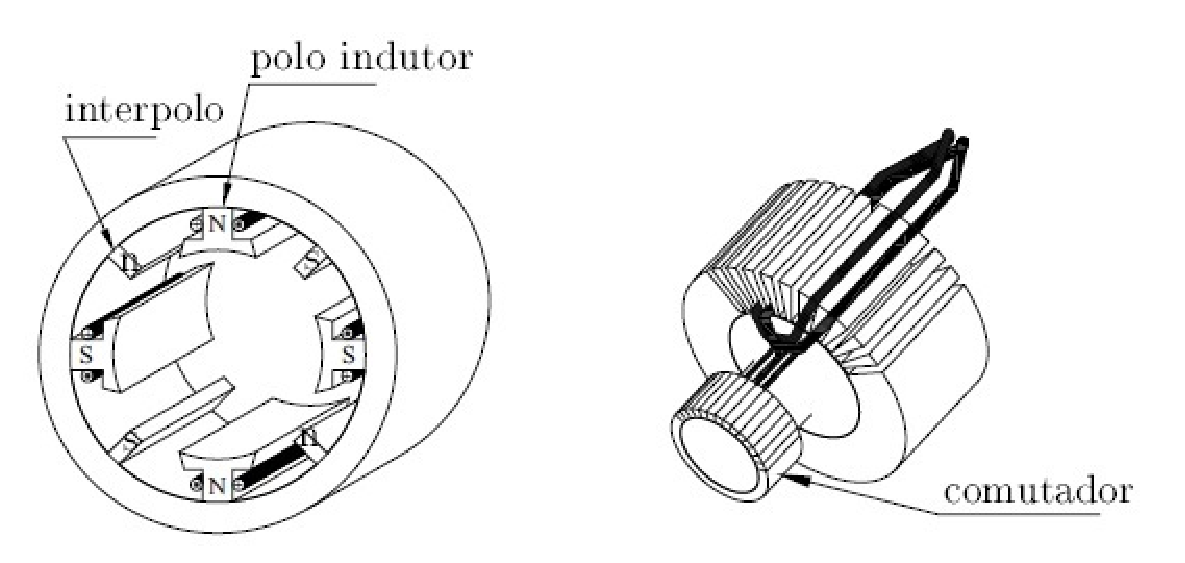
\includegraphics[width=\textwidth]{figuras/rotor.eps}
  \caption{Exemplo de um estator e um rotor \cite{bim}}
  \label{fig:rotor}
\end{figure}

\subsection{Dimensionamento Sistema Eletromecânico}

Para a análise das características requeridas de torque e potência foram estimados
massa do sistema foi estimada como $150 kg$, a sua velocidade máxima como $3 km/h$
e o tempo para atingir tal velocidade como $4$ segundos. A partir desses dados é
possível calcular a força necessária para colocar a cadeira em movimento bem como
para a acelerar até a velocidade máxima. Dividindo a velocidade pelo tempo necessário
para se alcançar a velocidade é possível calcular a aceleração.

$a =V/t =3/3.6*4= 0,20834 m/s2$

Em seguida calculamos a força necessária para acelerar a massa de $150 kg$.

$F_a=M * a =150 * 0,20834 = 31,25 N$

Também deve ser levado em conta a força necessária para colocar a massa da cadeira
em movimento, e usamos um valor de coeficiente de atrito estático $a = 0,3$.
$F_r=M*g* a = 441,45N$

Então a força total solicitada é dada pela soma da força de resistência ao movimento
e da força de aceleração.

$F_T=F_a+F_r=441,45+31,25 = 472,7 N$

Finalmente é possível calcular o torque solicitado utilizando o raio do eixo do
motor de $4mm$.

$T=F_T*R=472,7*0,004=1,8908 Nm$

A potência requerida é calculada multiplicando-se o torque pela velocidade máxima.

$P=T*V=441,45*0,83334 = 367 W$

\subsection{Especificações do Motor}

Serão utilizados dois motores da Bosch modelo GPB F006 KM0 611, que tem aplicações
em sistemas de arrefecimento, o emprego dos dois motores satisfaz as exigências
de potência e torque do sistema. As curvas características desse motor e seus
dados técnicos são mostrados a seguir.

\begin{figure}[H]
  \centering
    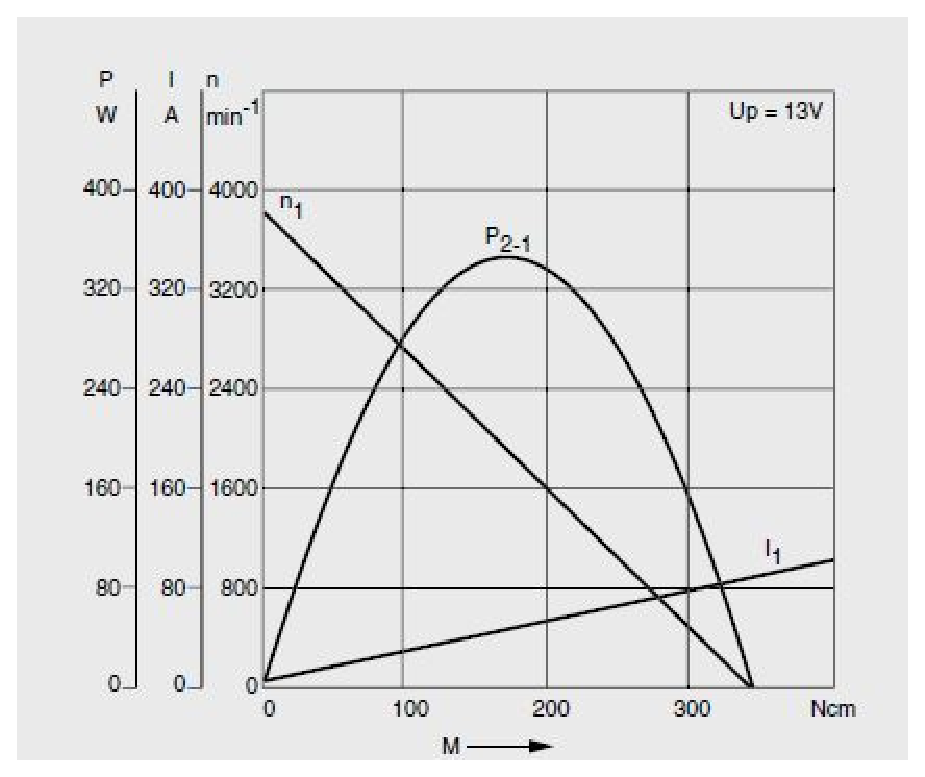
\includegraphics[width=\textwidth]{figuras/motor.eps}
  \caption{Curvas motor GPB F006 KM0 611 (Bosch)}
  \label{fig:motor}
\end{figure}

\begin{table}[h]
\centering
\vspace{0.5cm}
\begin{tabular}{|l|l|}
\hline
Item                & Especificação \\
\hline
Tensão Nominal      & 12 V \\
Potência Nominal    & 305 W \\
Rotação Nominal     & 2600 rpm \\
Corrente Nominal    & 25A \\
Torque Nominal      & 350 Ncm \\
Peso                & 1,585 kg \\
\hline
\end{tabular}
\caption{Dados motor GPB F006 KM0 611 (Bosch)}
\label{tab:dadosmotor}
\end{table}

\subsection{Dimensionamento da Bateria}

Sabe-se que a potência necessária para movimentar a cadeira de rodas é de $367 W$,
também sabe-se que a tensão nominal do motor GPB F006 KM0 611 da Bosch é de $12V$,
logo as baterias devem ser capazes de fornecer essa potência para o sistema por
pelo menos 3 horas. Para determinar qual bateria usar deve ser estimada a
capacidade em Ah, também devem as suas dimensões e peso, outro fator importante
é o custo, já que o projeto tem orçamento limitado \cite{costa}.

A bateria a ser utilizada deve ter uma tensão de $12V$, pois esse valor é
compatível tanto com a necessidade dos motores quanto com a disponibilidade dos
modelos de mercado. Tendo em vista a potência calculada e a tensão estabelecida
é possível calcular a corrente necessária.

$P = V*I$
$I = 367 W / 12 V =30,58 A$

Com esse valor de corrente e o tempo de trabalho do sistema é possível calcular
a carga da bateria.
$C = I * t= 30,58 * 3 =91,74 Ah$

Sabe-se que a bateria não deve ser totalmente descarregada, pois isso diminui a
vida útil da mesma, logo deve ser utilizado um fator de profundidade de descarga,
que nesse caso será de $80\%$ \cite{KARASINSKI}.

$C=91,74/0,8 = 114,675 Ah$

Um ponto importante no dimensionamento é o fato de o sistema de movimentação não
operar em plena carga a todo tempo, havendo momentos em que a potência necessária
é reduzida ou até mesmo nula, situação onde a cadeira está parada, portanto deve
se estimar um fator de demanda para os motores, para esse projeto o valor
adotado de para o fato de demanda será de $0,75$. Com isso temos que a carga
necessária será de:

$C=114,675 *0,75=86 Ah$

Uma possível solução que prioriza a variável custo é a utilização de $3$ baterias
de chumbo-ácido de $30 Ah$ ligadas em paralelo.



\section{Outros}

\subsection{Integração Contínua}
